\subsection*{Phylogenetic trees}

As we have already seen in that simple example of interaction between a biologist and a mathematician in the beginning of this chapter, the evolutionary history of a set of contemporary species is often modeled as a \emph{rooted phylogenetic tree}. Essentially, this is a rooted tree in which the leaves are bijectively labeled by the set of species and edges are directed away from the root, reflecting the direction of evolution \cite{SempleSteel2000}. Furthermore, the root represents the common ancestor of the set of species the tree is modeling and nodes of outdegree two or higher model the points in history at which a common ancestor of a subset of the species differentiated into two or more sublineages. The central problem in phylogenetics is to recover the topology of the ``true'' phylogenetic tree, given only information about the species, often DNA data. This is a challenging computational problem and has been the topic of intensive research during the last 40 years \cite{MathEvPhyl,reconstructingevolution,SemSte03}. 


Without further ado, denote the set of species (or more generally, \emph{taxa}) by $X$. A \emph{rooted phylogenetic $X$-tree $T$} is a rooted tree with no nodes with indegree~1 and outdegree~1, a root with indegree 0 and outdegree 2, and leaves bijectively labeled by the elements of $X$. Such a tree is called \emph{binary} if all inner nodes except the root have indegree~1 and outdegree~2. When some nodes have outdegree higher than 2, we speak of \textit{nonbinary} trees. We will encounter nonbinary trees in Chapter \ref{ch:3} and we postpone definitions of nonbinary concepts until then. For now we only talk of binary setting and we will refer to a rooted binary phylogenetic $X$-tree as a \emph{tree} for short. The edges of any rooted tree should be seen as being directed away from the root even though we will commonly draw them instead of arcs.

  %-----------------------------------------------------------------------------
  \begin{figure}[t]
    \centering
     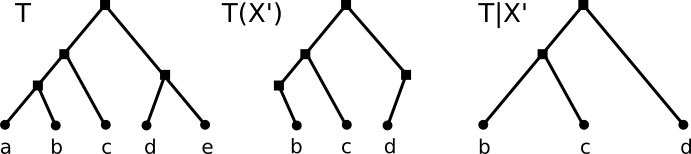
\includegraphics[width=0.7 \textwidth]{../figs/ch1/introtree.png}
    \caption{Let $X$ be a set of taxa $\{a,b,c,d,e\}$ and $X'$ its subset $\{b,c,d\}$. This figure shows an $X$-tree $T$, a minimal subtree of $T$ on $X'$ and a restriction of $T$ to $X'$.}
    \label{fig:introtree}
  \end{figure}
  %-----------------------------------------------------------------------------


The set of leaves of~$T$ is denoted as~$\cL(T)$. We identify each leaf with its label. In the course of this thesis, different types of subtrees play an important role. Let~$T$ be a rooted phylogenetic $X$-tree and~$X'$ a subset of~{$\cL(T)$}. The minimal rooted subtree of~$T$ that connects all leaves in~$X'$ is denoted by $T(X')$. Furthermore, the tree obtained from $T(X')$ by suppressing all {vertices with indegree and outdegree both equal to 1} is the {\it restriction of $T$ to $X'$} and is denoted by $T|X'$. See Figure \ref{fig:introtree}.

Let~$T$ be a rooted phylogenetic $X$-tree and~$S$ a rooted phylogenetic $X'$-tree for some $X' \subseteq X$. We say that~$S$ is a \emph{pendant subtree} of~$T$ if it is a subtree that can be detached from~$T$ by deleting a single edge. For a set~$\T$ of phylogenetic $X$-trees and $X' \subseteq X$, a \emph{common pendant subtree} of~$\T$ is a rooted phylogenetic $X'$-tree that is a pendant subtree of each tree in~$\T$. 

{
For $n\geq 2$, an {\it $n$-chain} of $T$ is an $n$-tuple $(a_1,a_2,\ldots,a_n)$ of elements of $\cL(T)$ such that the parent of $a_1$ is either the same as the parent of $a_2$ (see Figure \ref{fig:chains_ex} left) or the parent of $a_1$ is a child of the parent of $a_2$ (see Figure \ref{fig:chains_ex} right) and, for each $i\in\{2,3,\ldots,n-1\}$, the parent of $a_i$ is a child of the parent of $a_{i+1}$. The subgraph induced by $a_1,a_2,\ldots,a_n$ and their parents is called a {\em caterpillar}.
A \emph{common chain} of a set~$\T$ of trees is a maximal tuple $(x_1, x_2,...,x_q)$ that is a chain of each tree in~$\T$.
}

\begin{figure}[h]
 \centering
 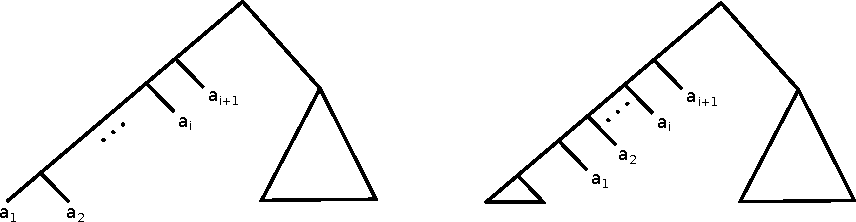
\includegraphics[width=0.9 \textwidth]{../figs/ch1/chains.pdf}
 \caption{Example of $n$-chains}
 \label{fig:chains_ex}
\end{figure}


However, our understanding of evolutionary mechanisms has deepened and there is growing awareness that evolution is not always treelike \cite{expanding}. In particular, due to \emph{reticulate phenomena} such as hybridizations, recombinations and horizontal gene transfer the evolution of a set of species is sometimes better modeled as a network rather than a tree \cite{davidbook}. Trees remain still equally relevant and they are often used as building blocks for networks.


\subsection*{Hybridization networks}
A \emph{rooted phylogenetic network} is essentially a generalisation of phylogenetic trees to directed acyclic graphs (DAGs). In such graphs nodes with indegree two or higher, known as \emph{reticulations}, represent the points at which two or more lineages merge, rather than diversify. 

Formally, a {\it rooted phylogenetic network $N$} on a set~$X$ is a rooted acyclic directed graph, which has a single root of outdegree 2, has no vertices with indegree and outdegree both~1, and in which the vertices of outdegree~0 are bijectively labelled by the elements of~$X$. A phylogenetic network is \emph{binary} if all vertices have indegree and outdegree at most~2 and every vertex with indegree~2 has outdegree~1. Intuitively we say that a phylogenetic network $N$ \emph{displays} a phylogenetic tree $T$ when all of the ancestral relationships visualized by~$T$ are visualized by~$N$. A precise definition will be given shortly. 

Following the publication of several seminal articles in 2004-5 (e.g. \cite{baroni05,BaroniEtAl2004}) there has been considerable research interest in the biologically-inspired question from the beginning of this chapter. Namely, given two rooted phylogenetic trees $T_1$ and $T_2$ on the same set of taxa $X$, what is the minimum number of reticulations required by a phylogenetic network $N$ on $X$ which displays both $T_1$ and $T_2$? This value is often called the \emph{hybridization number} in the literature, and when addressing this specific problem the term \emph{hybridization network} is often used instead of the more general term phylogenetic network. For the purpose of consistency we will henceforth use the term hybridization network. We now list some necessary definitions. 

For each vertex~$v$ of $N$, we denote by $d^-(v)$ and $d^+(v)$ its indegree and outdegree respectively. If $(u,v)$ is an arc of $N$, we say that~$u$ is a \emph{parent} of~$v$ and that~$v$ is a \emph{child} of~$u$. Furthermore, if there is a directed path from a vertex~$u$ to a vertex~$v$, we say that~$u$ is an \emph{ancestor} of~$v$ and that~$v$ is a \emph{descendant} of~$u$.

A vertex of indegree greater than one represents an evolutionary event in which lineages combined, such as a hybridization, recombination or horizontal gene transfer. We call these vertices \emph{hybridization vertices}. To quantify the number of hybridization events, the {hybridization number} of a (nonbinary) hybridization network $N$ is given by
$$h(N)=\sum_{v}(d^-(v)-1)$$
where $v$ goes over all vertices of $N$ except the root.
In a binary network, $h(N)$ is simply the number of vertices with indegree 2. Observe that $h(N)=0$ if and only if~$N$ is a tree.

Let $N$ be a hybridization network on~$X$ and~$T$ a rooted binary phylogenetic $X'$-tree with $X'\subseteq X$. We say that~$T$ is {\it displayed} by~$N$ if~$T$ can be obtained from~$N$ by deleting vertices and edges and suppressing vertices with $d^+(v)=d^-(v)=1$ (or, in graph-theoretic words, if a subdivision of~$T$ is a subgraph of~$N$). 

The problem {\sc MinimumHybridization}, abbreviated \mh, is to compute the {hybridization number} of two rooted binary phylogenetic $X$-trees~$T_1$ and~$T_2$, which is defined as
$$h(T_1,T_2)=\min\{h(N): N \mbox{ is a hybridization network that displays } T_1 \mbox{ and }T_2\},$$
i.e., the minimum number of hybridization events necessary to display two rooted binary phylogenetic trees.

This problem can be formulated as an optimization problem in the obvious way.\\

\noindent{\bf Problem:} {\sc MinimumHybridization}\\
\noindent {\bf Instance:} Two rooted binary phylogenetic $X$-trees $T_1$ and $T_2$. \\
\noindent {\bf Solution:} A hybridization network~$N$ that displays~$T_1$ and~$T_2$.\\
\noindent{\bf Objective:} Minimize $h(N)$.\\

If~$N$ is a hybridization network that displays~$T_1$ and~$T_2$, then there also exists a binary hybridization network~$N'$ that displays~$T_1$ and~$T_2$ such that $h(N)=h(N')$ \cite[Lemma~3]{twotrees}. Hence, we restrict our analysis to binary hybridization networks (even when we speak of nonbinary trees) and will not emphasize this again.


There is an interesting characterization of the hybridization number for two trees by another phylogenetic problem called Maximum Acyclic Agreement Forest, or \maaf for short. In this problem one is required to cut two input trees into common components, such that the number of components is minimized and there are no cyclical dependencies between them. In the next section we turn our attention to agreement forests and formally introduce this problem. 

%   %-----------------------------------------------------------------------------
%   \begin{figure}[t]
%     \centering
%     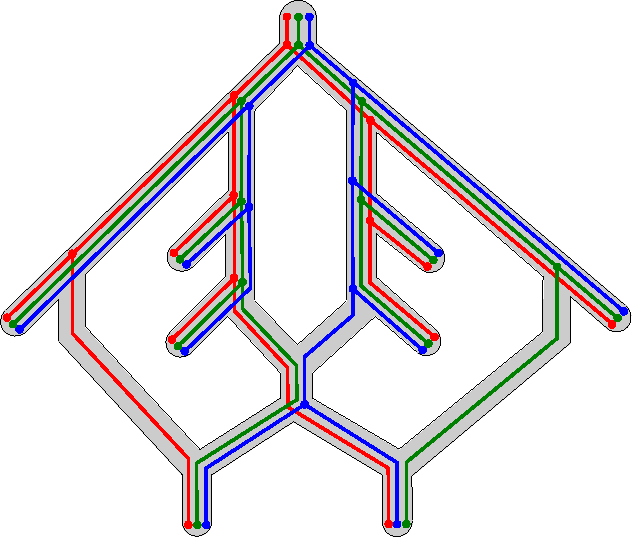
\includegraphics{../figs/ch1/introfig.pdf}
%     \caption{Network displaying three trees, red green and blue.}
%     \label{fig:intronet}
%   \end{figure}
%   %-----------------------------------------------------------------------------

{
A reader interested in the topic of phylogenetic networks, concepts and models that emerge in this area and their applications, is referred to 
\cite{HRS2011,surveycombinatorial2011,Nakhleh2009ProbSolv,Semple2007}.
}

\subsection*{Agreement Forests}

Let $T_1$ and $T_2$ be two rooted binary phylogenetic $X$-trees. Consider now a set of labels $X\cup\{\rho\}$, where $\rho$ is an additional leaf that we attach to the root of both trees $T_1$ and $T_2$. Or more precisely, since a root of any binary phylogenetic tree has outdegree two and indegree zero, we attach an edge to the root and label its  end by $\rho$. See figure \ref{fig:intromaaf}.


{A partition $\cF=\{\cL_\rho,\cL_1,\cL_2,\ldots,\cL_k\}$ of $X\cup\{\rho\}$ is an {\it agreement forest} for~$T_1$ and~$T_2$ if $\rho\in\cL_\rho$ and the following conditions are satisfied:}
\begin{itemize}
\item[(1)] for all $i\in\{\rho,1,2,\ldots,k\}$, we have $T_1|\cL_i \cong T_2|\cL_i$, and
\item[(2)] the trees in $\{T_1(\cL_i): i\in\{\rho,1,2,\ldots,k\}\}$ and $\{T_2(\cL_i): i\in\{\rho,1,2,\ldots,k\}\}$ are vertex-disjoint subtrees of $T_1$ and $T_2$, respectively.
\end{itemize}
In the definition above, the notation $\cong$ is used to denote a graph isomorphism that preserves leaf-labels.

Note that, even though an agreement forest is formally defined as a partition of the leaves $\cF=\{\cL_\rho,\cL_1,\ldots,\cL_k\}$, it is often useful to see it as a collection of trees $\cF=\{F_{\rho}, F_1,\ldots, F_k\}$ where $F_i=T_1|\cL_i$ (or equivalently $F_i=T_2|\cL_i$) for $i\in\{\rho,1,2,\ldots,k\}$. So, intuitively, an agreement forest for~$T_1$ and~$T_2$ can be seen as a collection of trees that can be obtained from either of~$T_1$ and~$T_2$ by deleting a set of edges and subsequently ``cleaning up'' by deleting unlabeled vertices and suppressing indegree-1 outdegree-1 vertices (see figure~\ref{fig:intromaaf}). Therefore, we often refer to the elements of an agreement forest as \emph{components}. The \emph{size} of an agreement forest~$\cF$ is defined as its number of elements (components) and is denoted by~$|\cF|$. 
{A natural optimization problem arises:}\\


\noindent{\bf Problem:} Maximum Agreement Forest (\maf)\\
\noindent {\bf Instance:} Two rooted binary phylogenetic $X$-trees $T_1$ and $T_2$. \\
\noindent {\bf Solution:} An agreement forest $\cF$ for $T_1$ and $T_2$. \\
\noindent {\bf Objective:} Minimize $|\cF|-1$ \\

%{It is not immediately obvious why we are minimizing the number of components minus one, but we come back to this shortly.}

The characterization of the hybridization number $h(T_1,T_2)$ in terms of agreement forests that we mentioned in the previous section requires an additional condition. Let $\cF=\{\cL_\rho,\cL_1,\cL_2,\ldots,\cL_k\}$ be an agreement forest for $T_1$ and $T_2$. Let $G_{\cF}$ be the directed graph that has vertex set $\cF$ and an edge $(\cL_i,\cL_j)$ if and only if $i\neq j$ and at least one of the two following conditions holds
\begin{itemize}
\item[(1)] the root of $T_1(\cL_i)$ is an ancestor of the root of $T_1(\cL_j)$ in $T_1$;
\item[(2)] the root of $T_2(\cL_i)$ is an ancestor of the root of $T_2(\cL_j)$ in $T_2$.
\end{itemize}
The graph $G_{\cF}$ is called the {\it inheritance graph} associated with $\cF$. We call $\cF$ an {\it acyclic agreement forest} for $T_1$ and $T_2$ if $G_{\cF}$ has no directed cycles. If~$\cF$ contains the smallest number of elements (components) over all acyclic agreement forests for $T_1$ and $T_2$, we say that $\cF$ is a {\it maximum acyclic agreement forest} for $T_1$ and $T_2$. Note that such a forest is called a \emph{maximum} acyclic agreement forest, even though one \emph{minimizes} the number of elements, because in some sense the ``agreement'' is maximized. (Also note that acyclic agreement forests were called \emph{good} agreement forests in~\cite{baroni05}.)

We define $m_a(T_1, T_2)$ to be the number of elements of a maximum acyclic agreement forest for~$T_1$ and~$T_2$ minus one. Also the problem of computing $m_a(T_1, T_2)$ has an optimization counterpart:\\


\noindent{\bf Problem:} Maximum Acyclic Agreement Forest (\maaf)\\
\noindent {\bf Instance:} Two rooted binary phylogenetic $X$-trees $T_1$ and $T_2$. \\
\noindent {\bf Solution:} An acyclic agreement forest $\cF$ for $T_1$ and $T_2$. \\
\noindent {\bf Objective:} Minimize $|\cF|-1$.\\


We minimize $|\cF|-1$, rather than~$|\cF|$, following~\cite{bordewich07a}, because $|\cF|-1$ corresponds to the number of edges one needs to remove from either of the input trees to obtain~$\cF$ (after ``cleaning up'') and because of the relation we describe below between this problem and {\sc MinimumHybridization}. Nevertheless, it can be shown that, from an approximation perspective, it does not matter whether one minimizes~$|\cF|$ or~$|\cF|-1$ (which is not obvious).

\begin{theorem}{\cite[Theorem 2]{baroni05}}\label{t:hybrid}
Let $T_1$ and $T_2$ be two rooted binary phylogenetic $X$-trees. Then
$$h(T_1,T_2)=m_a(T_1,T_2).$$
\end{theorem}


%--------------------------------------------------------------------------
\begin{figure}
    \centering
     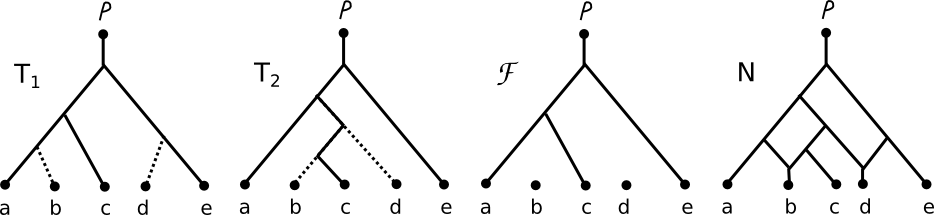
\includegraphics[scale=.5]{../figs/ch1/intromaaf.png}
    \caption{Two phylogenetic trees,~$T_1$ and~$T_2$, an acyclic agreement forest~$\cF$ for~$T_1$ and~$T_2$ with three components and its inheritance graph (which will later be drawn instead of that network). Forest~$\cF$ can be obtained from either of~$T_1$ and~$T_2$ by deleting the dashed edges.} 
    \label{fig:intromaaf}
\end{figure}
%--------------------------------------------------------------------------


